\scanpage{78}
$f$. For instance, using Chow's lemma and the Main existence theorem in my first talk on Picard schemes, one gets:

\uline{Corollary} 2\quad Assume $X/S$ proper satisfies the condition:\deleted{\unsure{a') for every}} \deleted{\unsure{any $X'$} \illegible{2} for} a') for every $X'$ finite over $X$, there \unsure{exist|exists} a non empty open subset $S_1$ of $S$ such that \inserted{\handwritten{problem A for}} $X'\handwritten{\mid}S_1$ has allways solution \deleted{for problems A and B} (this condition is satisfied if $X/S$ is projective). Then \deleted{there exists} provided we replace $S$ by a suitable $S_1$ non empty and open, $\underline{\mathrm{Pic}}_{X/S}$ exists, is separated, its connected components are of finite type over $S$.

N.B. The proof does not give any evidence towards the fact that in the theorem, one could replace ``quasi-affine'' by ``affine'' . This is true however over a \unsure{fièèd|fiéèd|field}, because a quasi-affine algebraic group is affine ! It would be interesting to have a couterexample, say,over a \deleted{valuation} ring of dimension $1$ such as $k\handwritten{[}t\handwritten{]}$ ,
\reversemarginpar
\margin{\handwritten{\figure{
\begin{tikzpicture}
\draw (0.22,0.10) arc[start angle=25,end angle=377,x radius=0.26cm,y radius=0.18cm];
\end{tikzpicture}}impossible if\\$X$ smooth !}}
\normalmarginpar
\figure{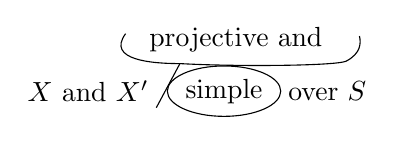
\begin{tikzpicture}[baseline=(simple.base)]
\node[anchor=east,inner sep=0pt] (xx) at (0,0) {$X$ and $X'$};
\node[inner sep=0pt] (simple) at (0.95,0) {simple};
\node[anchor=west,inner sep=0pt] at (1.76,0) {over $S$};
\node[inner sep=0pt] (projective) at (1.10,0.65) {\inserted{projective and}};
\handwritten{
\draw (simple.center) ellipse (0.72cm and 0.32cm);
\draw (0.09,-0.21) -- (0.39,0.35);
\draw (-0.30,0.73) .. controls (-0.55,0.39) and (0.05,0.35) .. (0.39,0.35)
 .. controls (1.10,0.31) and (2.35,0.32) .. (2.50,0.38)
 .. controls (2.69,0.48) and (2.69,0.61) .. (2.67,0.70);
}
\end{tikzpicture}}
and $X'\handwritten{\to}X$ birational,orr alternatively, \deleted{\unsure{if $X'$ finite}} $X$ and $X'$ projective and normal over $S$, and $f:X'\handwritten{\to}X$ finite. A counterexample in the latter case would of course provide a couterexample to the effectivity
% The following drawing retains the physical typed position of the moved words.
% The handwritten return line attaches the circled insertion before "raised".
\figure{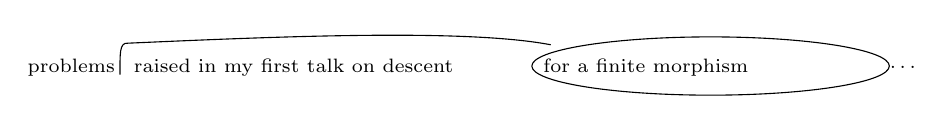
\begin{tikzpicture}[font=\scriptsize]
\node[anchor=west,inner sep=0pt] (problem) at (0,0) {problem\deleted{\unsure{s}}};
\node[anchor=west,inner sep=0pt] (raised) at (1.35,0) {raised in my first talk on descent};
\node[anchor=west,inner sep=0pt] (morphism) at (6.55,0) {\inserted{for a finite morphism}};
\node[anchor=west,inner sep=0pt] at (10.95,0) {\dots};
\handwritten{
\draw (8.68,0.02) ellipse (2.27cm and 0.37cm);
\draw (6.65,0.29) .. controls (5.55,0.50) and (3.10,0.39) .. (1.28,0.31)
 .. controls (1.17,0.32) and (1.18,0.18) .. (1.18,-0.09);
}
\end{tikzpicture}}

``Problem A'' is the following: given $X/S$ and \deleted{any} Module $F$ on $X$, to represent the functor on the category of $S$-preschemes taking any $S'/S$ into \deleted{the empty or} into a one-element \inserted{or into the empty} set; according as to wheter $F'$ on $X'/S'$ is flat with respect to $S'$\inserted{\handwritten{or not}}, where $X'=X\mathbin{x}_S S'$, $F'=F\unsure{2|x|\otimes}_S S'$ . Given $X/S$, we say that ``Problem A \inserted{\handwritten{for $X/S$}} has always a solution'' if for every coherent $F\handwritten{'}$ on \deleted{\unsure{$X$}}\inserted{\handwritten{some $X'/S'$}}, the previous functor \inserted{\handwritten{on $(\mathrm{Sch})/S'$}} is representable by a \inserted{$S\handwritten{'}$\handwritten{-}}scheme of finite type. The main step in my proof of existence of Hilbert schemes shows that this condition is satisfied when $X/S$ is projective,
% archive sheet number: 77
